\section[Das Tablet-Layout (Jürgen Hetzel)]{Das Tablet-Layout
\begin{tiny} (Jürgen Hetzel)\end{tiny}}

Tablets stellen mehr Fläche für die Elemente der \emph{Activities} zu Verfügung. Infolgedessen muss diesem Umstand Rechnung getragen werden.
Auf Grund diverser Tests, wurde die Entscheidung getroffen, den Portrait-Modus für Tablets (7 sowie 10 Zoll) nicht zu verändern. Bei einer horizontalen Aufteilung des vorhandenen Platzes im Portrait-Modus, würde der Chart unverhältnismäßig klein erscheinen.

Ferner wurden Überlegungen bezüglich der Darstellung der Fragmente angestellt. Der Chart wird in dieser Ansicht leider nicht angezeigt, da dieser erst zur Laufzeit sichtbar wird. Er befindet sich unterhalb der Überschrift \emph{Beschleunigungssensor}. 
Bei einer Positionierung der Fragmente \emph{DeviceMap} und \emph{Info} nebeneinander, erscheint die Karte in Relation zur Displaygröße, zu klein.
Zudem wäre es für den Benutzer erforderlich, innerhalb des Info-Fragments vertikal zu scrollen. Das \emph{Swipen} auf die Map, erscheint hingegen weniger unangenehm. Folglich wurde ein Lösung gewählt, bei der auf das Scrollen inmitten des Info-Fragments verzichtet werden kann, die Karte jedoch komfortabel groß erscheint und die gesamte Display-Größe genutzt wird.

\begin{figure}[H]
\centering
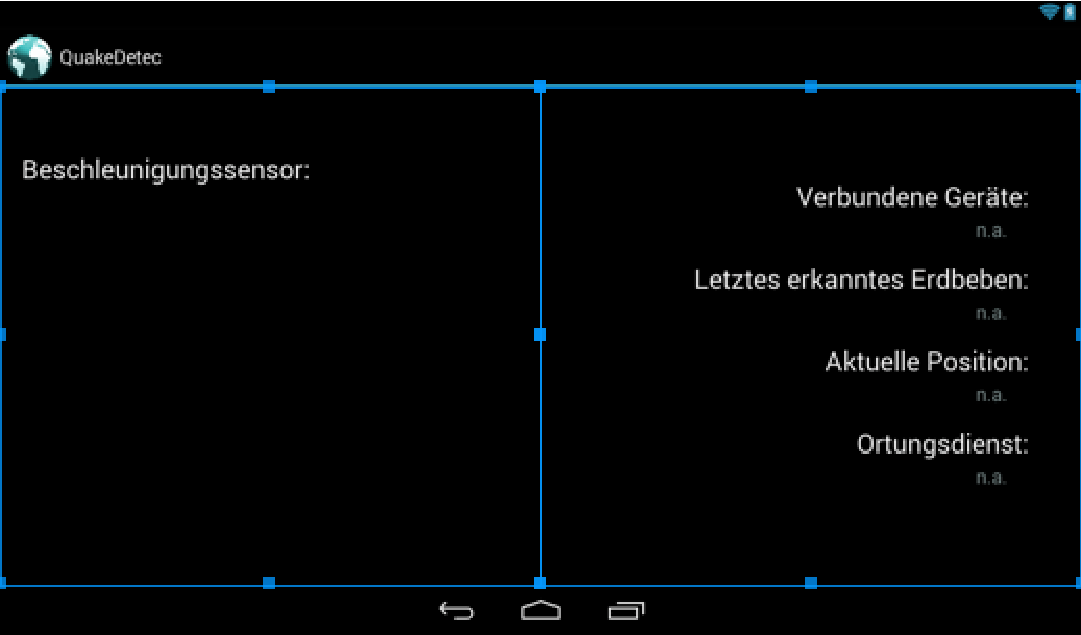
\includegraphics[width=\textwidth]{/TabletLayoutPos.pdf}
\caption{Die Anordnung der Elemente des Tablet-Layouts}
\label{fig:TabletLayoutPos}
\end{figure}

Abbildung \ref{fig:TabletLayoutPos} zeigt die Aufteilung des Tablet-Layouts im Landscape-Modus.
Mittels \emph{Relative Layout} werden die einzelnen Elemente relativ zueinander positioniert und zentriert. Für die horizontale Anordnung werden \emph{LinearLayouts} verwendet und der verfügbare Platz zu gleichen Teilen, zwischen Informationen und Chart, aufgeteilt, um so ein stimmigeres Gesamtbild zu vermitteln. Mit einer Aufteilung gemäß goldenem Schnitt (Verhältnis x1: x2 entspricht ungefähr 1,62) wurden schlechtere Ergebnisse im Hinblick auf den Gesamteindruck erzielt. Für die Darstellung der Informationen sowie Chart und Überschrift, bieten sich vertikale Listen an. Der Abstand von der Chart-Ordinate bezüglich des Seitenrands entspricht dem der Informationen. Infolgedessen bleibt die Symmetrie gewahrt.




